\section{Requirements}
The first requirements that are needed in order to develop the big data application is to install the corresponding versions of Eclipse, Papyrus and Acceleo. In spite of the application is able to work with other versions, some problems could appear because of the changes that they present. The models implemented in this document have been developed with the following versions:

\begin{itemize}

\item Eclipse 2019-03 (4.11.0).
\item Papyrus SysML 1.4 Feature	1.3.0.
\item Acceleo 3.7.8.201902261618.
\item m2e-Maven Integration for Eclipse (includes Incubating components) 1.11.0.20190220-2119.
\item Apache Flink 1.4.0.

\end{itemize}

\section{Design}
\subsection{Great Seller DIA}
Along this document a DIA for an e-commerce company called Great Seller is implemented. This DIA is able to compute real time statistics about the transactions generated by the consumers. Such statistics can be observed by some other companies that pay in order to have access to the information making that Great Seller acts as a data broker. In order to simplify the implementation, Great Seller is going to sell three different types of statistics:

\begin{itemize}

\item Statistic 1: the total amount of money that each consumer of Great Seller spend in the last 10 minutes.
\item Statistic 2: the number of transactions issued by each user in the last 10 minutes.
\item Statistic 3: the number of users who spent more than \euro{1000} in the last hour.

\end{itemize}

As any DIA, Great Seller generates such statistics by some transformations which are fed from a source and the generated information is stored into a sink which is accessible by the observer companies. Moreover, as Great Seller is producing three different types of statistics, its DIA requires three different sinks where the information should be stored. Due to the fact that Great Seller DIA is computing real time statistics about the transactions that are generated by the consumers of the company, only one source is required for the DIA model. Finally, one transformation is necessary for the computation of each statistic. In summary, Great Seller DIA requires one source, three transformations and three sinks for the design of its model.

\subsubsection{Great Seller Source}
In the implementation described along this document, Great Seller DIA is fed from a text file where all the transactions generated by the consumers of Great Seller are stored. All the transactions are going to have the same predefined tuple structure 'transactionId,dataSubject,spentAmount,purchasedProduct'. This predefined structure is represented in the Great Seller DIA model by means of a Data Type called InputTransaction.

Regarding to the fields of such tuple, the transactionId field is an integer which varies from 1 to the number of generated transactions, such number can be 10, 100 or 1000. The dataSubject is the user who generates such tuple and it is one of the following: Bob, Carlos, Elisabetta or Michele. The spentAmount is the price paid for the product bought with the transaction and it is an integer with a low boundary of \euro{1} and an upper boundary of \euro{200}. Finally, the purchasedProduct is the product bought with such transaction.

The Great Seller stock is composed by means of 25 products. In order to simplify the implementation, each product is named by the word 'product' immediately followed by a number between 1 and 25 in order to specify the product referred in the stock. In the table \ref{Great Seller Stock} can be seen such stock.

\begin{table}[h!]
\centering
	\begin{tabular}{||c|c||} 
	\hline\hline
	Product & Price (\euro{}) \\ [1ex] 
	\hline\hline
	product1 & 196 \\ 
	\hline
	product2 & 36 \\ 
	\hline
	product3 & 179 \\ 
	\hline
	product4 & 17 \\ 
	\hline
	product5 & 120 \\ 
	\hline
	product6 & 187 \\ 
	\hline
	product7 & 139 \\ 
	\hline
	product8 & 52 \\ 
	\hline
	product9 & 160 \\ 
	\hline
	product10 & 110 \\ 
	\hline
	product11 & 113 \\ 
	\hline
	product12 & 67 \\ 
	\hline
	product13 & 100 \\ 
	\hline
	product14 & 125 \\ 
	\hline
	product15 & 192 \\ 
	\hline
	product16 & 115 \\ 
	\hline
	product17 & 113 \\ 
	\hline
	product18 & 98 \\ 
	\hline
	product19 & 113 \\ 
	\hline
	product20 & 185 \\ 
	\hline
	product21 & 143 \\ 
	\hline
	product22 & 18 \\ 
	\hline
	product23 & 194 \\ 
	\hline
	product24 & 41 \\ 
	\hline
	product25 & 26 \\ 
	\hline\hline
	\end{tabular}
\caption{Great Seller Stock}
\label{Great Seller Stock}
\end{table}

\subsubsection{Great Seller Transformations}
In order to compute each of the three statistics that Great Seller sells as data broker, the Great Seller DIA needs three transformations. Each of this transformations is the operator of each statistic. Thus, the operator one (OP1) computes the total amount of money spent by each user in the last 10 minutes. The second operator (OP2) computes the number of transactions issued by each user in the last 10 minutes. Finally, the operator three (OP3) computes the number of users who spent more than \euro{1000} in the last hour.

These transformations input a data stream with a set of tuples that all of them have identical structure. Thus, the first stream (S1) is composed of tuples of the kind InputTransaction. This stream is duplicated and it is sent to the operators OP1 and OP2. Moreover, as each operator works taking into account the data subject of each tuple, the stream S1 must be keyed by the data subject field of this first stream. Finally, as the operators have to compute the statistics taking into account only the tuples generated in the last 10 minutes, the stream S1 is windowed by a time window of 10 minutes.

The new data generated in the OP1 are represented in a new data type called SpentAmount and that is composed by two fields following the structure: 'dataSubject, totalAmount'. The SpentAmount tuples are collected in the stream S2 and they are keyed by the data subject field of such stream.

Finally, the data generated in the OP2, is collected in a new data type called IssuedTransaction whose structure is 'dataSubject, nTransactions'. This new stream (stream S3) is sent to the OP3. Moreover, this third stream is keyed by the data subject field of the stream and it is also windowed with a time window of one hour. The OP3 generates a randomly partitioned stream with an uniform distribution called stream S4 whose structure is: 'nTopUsers'.

\subsubsection{Great Seller Sinks}
Each of the tuples flowing through the DIA must be stored in a file, in order to be able to access to the tuples that will be sent to the observer companies. This is why, after each generated stream, a file text sink is implemented with different paths in order to store each of the flows obtaining all the results in three different files. The file with the results of the stream S2, the stream S3 and the stream S4.
This implementation is given due to the fact that each of the tuples generated by the operators are observable for the observer companies who buy them.


In the figure \ref{fig:Great Seller DIA} the dataflow model of the Great Seller DIA without privacy policies can be seen.

\begin{figure}
\centering
{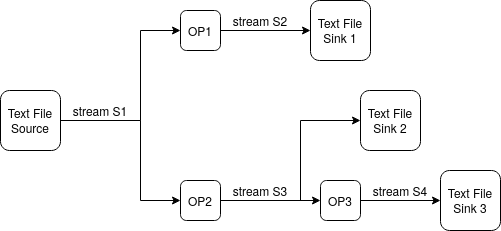
\includegraphics[scale=0.5]{./chapter3/greatSellerApp.png}}
\caption{Great Seller DIA}
\label{fig:Great Seller DIA}
\end{figure}















